\chapter{Grand Truth Generation: Fitting a Circle (initial approach)}

\section{Introduction}
The objective of this chapter is to present the initial 
approach developed for generating ground truth data to 
estimate the 3D location and orientation of a steering wheel 
using 2D and 3D geometric techniques. This approach sought 
to capture the steering wheel’s geometric structure by 
fitting a 2D ellipse to the annotated points and extending this 
representation into 3D space through additional processing 
steps.


Given the complexity of manually annotating the steering wheel 
across numerous images and the inherent sparsity and noise in 
the data, the annotation process is automated and enganced by fitting a mathematical model to a few number of 
spars annotations. This model would allow us to generate a 
more comprehensive representation of the steering wheel 
geometry.
The approach was divided into several phases:
\begin{enumerate}
    \item Annotating the steering wheel with 2D points.
    \item Fitting an ellipse to the annotated 2D points.
    \item Sampling additional points from the ellipse and mapping them into 3D space.
    \item Fitting a sphere to the 3D points to refine the geometry.
    \item Deriving a circular cross-section from the sphere to better represent the steering wheel.
\end{enumerate}

Although this initial approach showed some promise, it was 
constrained by the sparse and noisy nature of the data, 
resulting in a lack of precision in the final 3D representation 
of the steering wheel. Furthermore, there was no systematic 
method to effectively evaluate the ground truth data accuracy 
generated by this approach.

This chapter details the methodology, results, and the reasons 
for transitioning to a more reliable approach.


\section{Methodology}

\subsection{Annotating the Steering Wheel with 2D Points}
The process began with manual annotation of the steering wheel 
in 2D images. Annotating a dense and accurate set of points 
across all images was infeasible due to the time-consuming 
nature of manual annotation and the large number of frames. 
Hence, a sparse set of 2D points was initially marked to 
provide a basic outline of the steering wheel as depicted in 
\cref{fig:ellipse}.

\subsection{Fitting an Ellipse to 2D Points}
In order to create a denser representation, an ellipse was fitted to the existing 2D annotation points. This provided 
a more complete 2D shape that captured the true geometric 
structure of the steering wheel as illustrated in \cref{fig:ellipse}. 

The ellipse was fitted to these points using the general equation of an ellipse:
\[
c_0 X^2 + c_1 XY + c_2 Y^2 + c_3 X + c_4 Y = b
\]
To find the coefficients \([c_0, c_1, c_2, c_3, c_4]\) 
that best fit to the observed points \((X, Y)\), linear 
regression was applied. Defining \( A = [X^2, XY, Y^2, X, Y] \) and 
\( c = [c_0, c_1, c_2, c_3, c_4] \), the coefficients are calculated 
by solving for \( c \) that satisfies the equation \( Ac = b \), 
where \( b \) represents the constant in the ellipse equation. 


\subsection{Sampling Points from the Ellipse and Mapping to 3D}
Once the ellipse was fitted, 1000 points were sampled from 
the ellipse and its neighboring regions to create a denser 
representation as shown in \cref{fig:sampled_points}. These points were mapped from 2D to 3D using 
depth information from the camera and the intrinsic parameters.

However, due to the sparse and noisy nature of the data, 
the sampled points could not accurately represent the true 
geometry of the steering wheel, resulting in an inaccurate 
approximation of the 3D position and orientation. 
As depicted in \cref{fig:obb}, the bounding box fitted to the 
mapped 3d points was unable to accurately represent the 
position of the steering wheel.

\subsection{Fitting a Sphere to the 3D Points}
To further refine the 3D representation, a sphere was fitted to the sampled points on the steering wheel as demonstrated in
\cref{fig:sphere}. 
Given the sample points \((x, y, z)\), the general 
equation of a sphere is as following:
\[
(x - h)^2 + (y - k)^2 + (z - m)^2 = r^2
\]
Expanding this equation obtains:
\[
x^2 + h^2 - 2xh + y^2 + k^2 - 2yk + z^2 + m^2 - 2mz = r^2
\]
Rearranging terms yields:
\[
2xh + 2yk + 2zm + (r^2 - h^2 - k^2 - m^2) = x^2 + y^2 + z^2
\]
Letting \( A = [2x, 2y, 2z, 1] \), \( c = [h, k, m, r^2 - h^2 - k^2 - m^2] \), and 
\( b = x^2 + y^2 + z^2 \), a sphere can fit to the points by solving for \( c \) in the equation:
\[
Ac = b
\]

This solution provides us with the center \((h, k, m)\) and radius 
\(r\) of the sphere.


\subsection{Refining with a Circular Cross-Section from the Sphere}
To better capture the essential structure of the steering wheel, a circular cross-section of the fitted sphere in the XY plane was taken by fixing \( z = m \). This simplification was based on the observation that the steering wheel’s geometry is primarily defined in the XY plane, with minimal variation along the z-axis. 
Principal Component Analysis (PCA) of the steering wheel points 
revealed that the distribution along the z-axis is very limited, 
indicating that this axis does not contain significant information 
about the overall shape or structure of the steering wheel. 
By constraining the representation to the XY plane, unnecessary complexity from minor variations along 
the z-axis was avoided, which could detract from the accuracy of the wheel’s positioning.

This circular cross-section represented the X and Y 
correlations in the steering wheel geometry, 
simplifying the model while preserving the essential spatial 
characteristics of the wheel.


\subsection{Aligning the Circle with a Rotation Matrix}
Finally, this circle was aligned to the steering wheel’s position 
by applying a rotation matrix followed by a translation 
to center of the sphere. The rotation matrix was derived 
from the oriented bounding box of the steering wheel 3D points 
illustrated in \cref{fig:obb}. Open3D OrientedBoundingBox method 
\footnote{available at \url{http://www.open3d.org/docs/release/python_api/open3d.geometry.OrientedBoundingBox.html}}
was employed to compute the orientation and rotation matrix, 
which allowed us to align the circle with the steering 
wheel’s orientation in 3D space. 
Figure \cref{fig:circle} shows the final circular representation of the steering wheel's 3D position.

\begin{figure}[ht]
    \centering
    \begin{subfigure}[t]{0.18\textwidth}
        \centering
        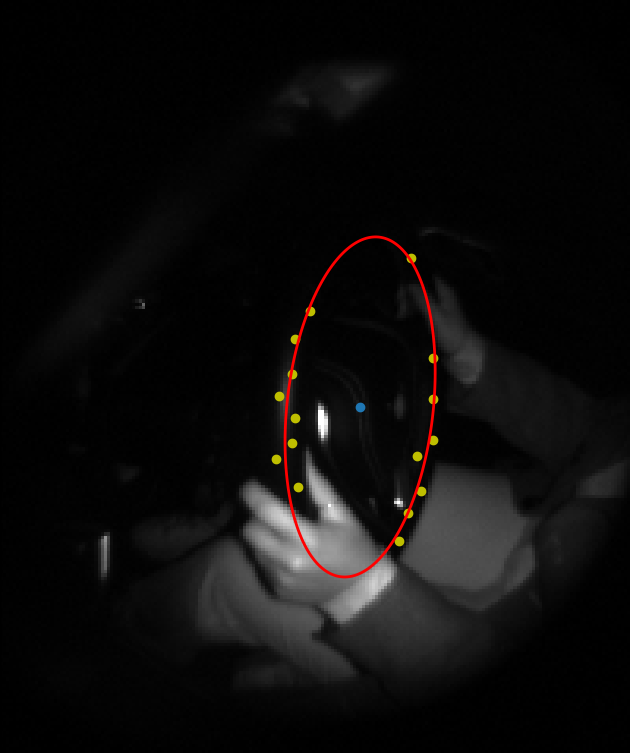
\includegraphics[width=\textwidth]{media/chapter 4/ellipse.png}
        \caption{}
        \label{fig:ellipse}
    \end{subfigure}\hfill
    \begin{subfigure}[t]{0.18\textwidth}
        \centering
        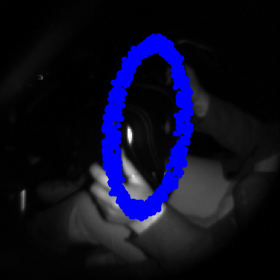
\includegraphics[width=\textwidth]{media/chapter 4/sampled_points.png}
        \caption{}
        \label{fig:sampled_points}
    \end{subfigure}\hfill
    \begin{subfigure}[t]{0.18\textwidth}
        \centering
        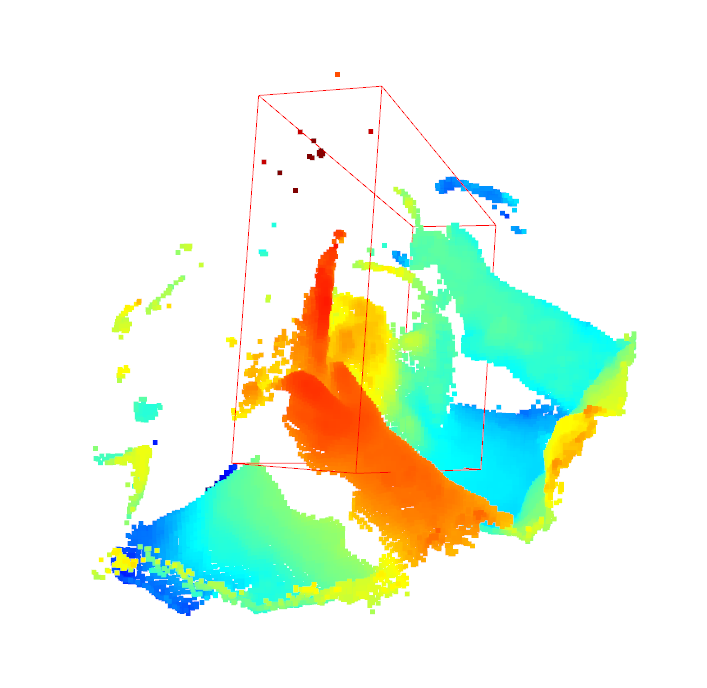
\includegraphics[width=\textwidth]{media/chapter 4/obb.png}
        \caption{}
        \label{fig:obb}
    \end{subfigure}\hfill
    \begin{subfigure}[t]{0.18\textwidth}
        \centering
        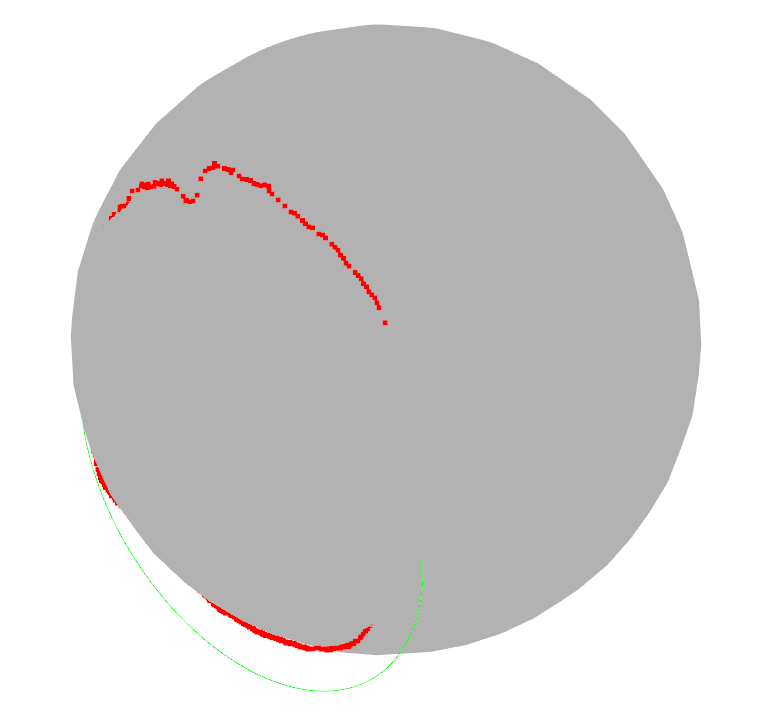
\includegraphics[width=\textwidth]{media/chapter 4/sphere.png}
        \caption{}
        \label{fig:sphere}
    \end{subfigure}\hfill
    \begin{subfigure}[t]{0.18\textwidth}
        \centering
        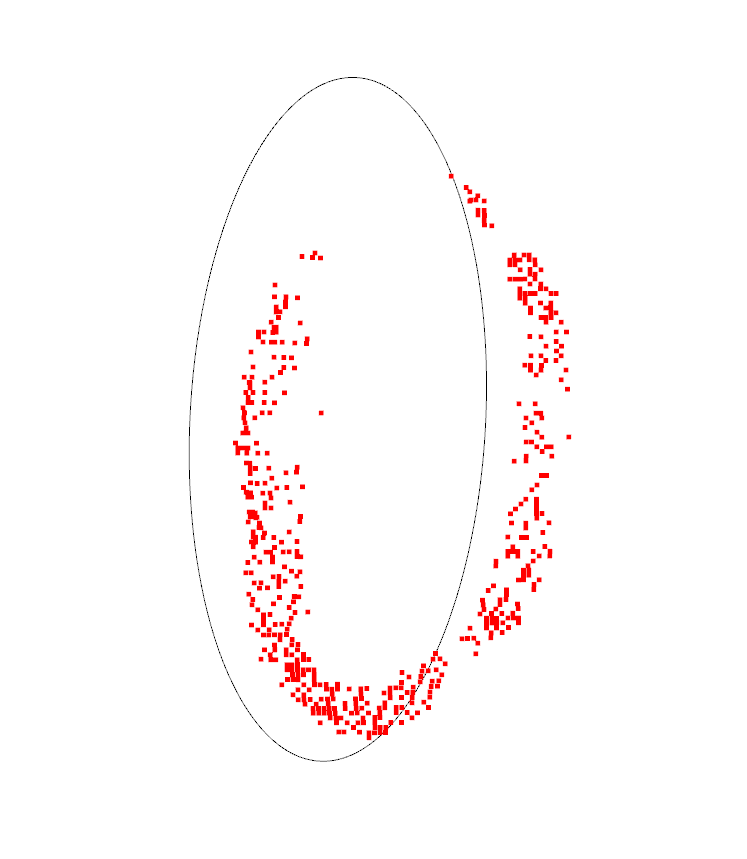
\includegraphics[width=\textwidth]{media/chapter 4/circl.png}
        \caption{}
        \label{fig:circle}
    \end{subfigure}\hfill
    \caption{(a) Steering wheel annotated with 2d points 
    and an ellipse fitted to the 2D points. (b) 1,000 points were sampled from the ellipse 
    and its small neighborhood.(c) The sampled points were mapped to 3D space, 
    with the bounding box illustrating these points in 3D. 
    (d) A sphere was fitted to the sampled points. 
    (e) The 3D model was refined by deriving a 
    circular cross-section from the sphere, representing 
    the steering wheel’s 3D position as a circle in 
    3D space.}
\end{figure}


\section{Conclusion}
Despite these steps, this approach was ultimately limited by the sparse and noisy data, as well as the lack of an accurate evaluation method 
for the generated ground truths. This made it difficult to ensure the 
precision of the ground truths in accurately capturing the true location and orientation of the 
steering wheel. These limitations prompted us to pursue a second 
approach using ArUco board for more reliable results.

